\documentclass[12pt]{article}
\usepackage[utf8]{inputenc}
\usepackage[french]{babel}
\usepackage{graphicx}
\usepackage[T1]{fontenc}
\usepackage{lmodern}
\usepackage{amsmath}
\usepackage{amsfonts}
\usepackage{amssymb}
\usepackage{ifthen}
\usepackage{multicol}
\usepackage{fancyhdr}
\newcommand{\marge}{18mm}
\usepackage[left=\marge,right=\marge,top=\marge,bottom=\marge]{geometry}
\pagestyle{fancy}
\setlength{\headheight}{14pt}
%	\chead{\ifthenelse{\thepage=1}{
%	 \textbf{Nom :}
%	  \makebox[12em]{\dotfill}
%	  \hspace{2em}
%	  \textbf{Pr\'enom :}
%	  \makebox[12em]{\dotfill}}{}}
\rfoot{\ifthenelse{\thepage=1}{\textit{(tournez la page s.v.p)}}{}}
\renewcommand{\headrulewidth}{0pt}
\linespread{1.3}
\setlength{\columnseprule}{0.2pt}
 
% Commandes sp\'ecifiques pour les QCM
\newboolean{correction}
% true pour afficher la correction
% false pour la masquer
\setboolean{correction}{false}
\newcounter{QNumber}
\newcommand{\Question}[2][ ]{
 \stepcounter{QNumber}
  \noindent\textbf{Question \theQNumber} --
  #2~#1}
\newenvironment{Reponse}{
 \begin{list}{$\square$}{\leftmargin=4em}}{
 \end{list}\vspace{1em}}
\newcommand{\Vrai}{
 \item[\ifthenelse{\boolean{correction}}{$\blacksquare$}{$\square$}]}
\newcommand{\Faux}{\item[$\square$]}
 
\def\N{\mathbb N}
\def\R{\mathbb R}
\def\Q{\mathbb Q}
\def\Z{\mathbb Z}
\begin{document}
  \begin{center}
    \bfseries\LARGE
    \textit{INFO I31, partiel, 18 Nov 2014}\large
  \end{center}
  \sffamily
%	\begin{itshape}
%	Pour chaque question, r\'epondez directement sur la feuille.
%	Quand vous avez le choix, il n'y a qu'une seule bonne r\'eponse par question. Lisez et comprenez les questions avant d'y r\'epondre~!
%	  \end{itshape}
%%\begin{multicols}{1} %%\begin{multicols}{2}
\setlength\parskip{0.2cm} 

\noindent {\bf RÉPONDEZ AUX 23 QUESTIONS DANS L'ORDRE~;  MENTIONNEZ LE NUMÉRO DE LA QUESTION DEVANT CHAQUE REPONSE (EVENTUELLEMENT VIDE).} 
%~\\

\noindent {\bf VOUS AVEZ DROIT A TOUS VOS DOCUMENTS PERSONNELS. }
%~\\

\noindent {\bf TOUT INSTRUMENT ELECTRONIQUE EST INTERDIT. }
%~\\

\noindent {\bf ECRIVEZ LISIBLEMENT. MERCI !}
%~\\

\noindent {\bf IL Y A 23 QUESTIONS, NUMEROTEES DE 1 A 23.}
~\\

\Question{D\'eroulez l'algorithme d'Euclide pour calculer le PGCD de 325 et 240 (en utilisant la division euclidienne, et pas la soustration).
Dans la dernière ligne, $a$ ou $b$ est nul, et la case  $r$ est vide.
Entourez la valeur du pgcd. Le tableau solution  a 7 lignes (sans compter la ligne $a, b, r$).}

\noindent{\bf Réponse}~:

$$
\begin{array}{|c|c|c|}
\hline
\; a\; & \; b\; & \; r\; \\
\hline
325 & 240 & 85 \\
240 &  85 & 70 \\
85  &  70 & 15 \\
70  &  15 & 10 \\
15  &  10 & 5 \\
10  &  5  & 0 \\
5   &  0  & \_  \\  
\hline
\end{array}
$$
Donc pgcd$(325, 240)=5$

\Question{Soient $a \ge b > 0$ deux entiers donnés. L'algorithme d'Euclide étendu 
calcule $g$ le PGCD de $a$ et $b$ ainsi que les plus petits entiers $u$, $v$ tels que $au+bv=g$. Dans la programmation récursive, la fonction est récursivement appelée sur $a'=b$, et $b'=a \mod b$; elle rend $g'$, $u'$ et $v'$ tels que
$a'u'+b'v'=g'=\mbox{PGCD}(a',b')$. Donnez, sans démonstration,  les formules
pour calculer  $g, u, v$ en fonction de $g', u', v'$. Vous pouvez utiliser $q$ le quotient (entier) de $a$ par $b$.}

\noindent{\bf Réponse}~:

$g=g', u=v', v=u'-q\times v$. 

Preuve (non demandée): soient  $a$ et $b$ 
deux entiers naturels  donnés;  on suppose que $a\ge b$.  Il faut calculer
Bezout$(a,b)$= $(u,v,g=\mbox{pgcd}(a,b))$ tels que $au+bv=g$.
Si $b=0$, alors $(u, v, g)=(0, 1, b)$ est une solution (n'importe quelle valeur de $u$ convient, puisque $a=0$). Sinon, soient $r, q$ tels que $r=a \mod b$ et $a=bq+r$ (il est possible de prendre $r$ non négatif dans $[0, b-1]$,
ou bien dans $[- b/2, (b+1)/2]$ comme Gauss si bien que $|r| \le b/2$); soit Bezout$(b, r= a \mod b)=(u',v',g')$.
Donc 
$$bu' + rv'=g'\Rightarrow b u' + (a-bq) v' = g' \Rightarrow av' + b(u'-qv')=g'$$
Une solution possible pour $(u,v,g)$ est donc $(v', u'-qv', g')$.
D'autres solutions sont $(u+tb,v-ta,g)$ pour tout $t$ entier.

\Question{D\'eroulez l'algorithme d'Euclide \'etendu (ou Bézout) pour $a=325$ et $b=240$.
$u$ et $v$ sont tels que $au+bv=g=PGCD(a,b)$; $r=a \mod b$, et $q=\lfloor \frac{a}{b}\rfloor$
est le quotient entier de la division de $a$ par $b$}
Dans la dernière ligne, $a$ ou $b$ est nul, et les cases $q$ et $r$ sont vides.
$$
\begin{array}{|c|c|c|c||c|c|c|}
\hline
\; a\; & \; b\; & \; r\; & \; q\; & \; g\; & \; u\; & \; v\; \\
\hline
325 & 240 & 85 &  1  &  5 &  17 & -23 \\
240 & 85  & 70 &  2  &  5 &  -6 & 17 \\
85  & 70  & 15 &  1  &  5 &  5 & -6  \\
70  & 15  & 10 &  4  &  5 &  -1 & 5 \\
15  & 10  & 5  &  1  &  5 &  1 & -1 \\
10  & 5   & 0  &  2  &  5 &  0 & 1 \\
5   & 0   & \_  &  \_  &  5  &  1 & 0 \\
\hline
\end{array}$$

\Question{Citez les noms de 3 algorithmes optimaux de tri}

\noindent{\bf Réponse}. Tri par fusion (mergesort), tri par tas (heapsort), tri rapide (quicksort)  probablement optimal, tri par insertion dans un arbre binaire équilibré (AVL, 2-3 arbre, b-arbre, etc).

{
\Question{Un \'etudiant programme une m\'ethode de tri. Son programme met 1 seconde pour trier 100 mille \'el\'ements ($10^5$),
et 4 secondes pour trier 200 mille \'el\'ements ($2\times 10^5$).
Notons $n$ le nombre d'\'el\'ements \`a trier.  La complexit\'e de son algorithme est en~?}

\noindent{\bf Réponse}. Le temps de traitement est multiplié par 4 quand le nombre d'éléments est multiplié par 2. Le programme est donc en $O(n^2)$.
}

{
\Question{Quel est l'ordre de grandeur du nombre de comparaisons effectu\'ees par un algorithme optimal de tri (qui  n'utilise que des comparaisons entre 2 \'el\'ements) }
}

\noindent{\bf Réponse}; $O(n\log n)$. Principe de la preuve: chaque comparaison permet, dans le meilleur des cas, d'éliminer la moitié des ordres possibles a priori. Il y en a $n!$ au départ (factorielle de $n$). Donc il faut au minimum $\log_2(n!)$ comparaisons. Or $\log(n!)= \log(1)+\log(2)+\ldots \log(n)= O(n\log n)$

{
\Question{Donnez les formules n\'ecessaires pour le calcul r\'ecursif 
de $a^n$ ($a\in \R, n\in\N$). N'oubliez pas le ou les cas terminaux.}  
}

\noindent{\bf Réponse}. $a^0=I$, $a^{2k}=(a^2)^k$, $a ^{2k+1}=a\times (a^{2k})$. Donc $\log_2 n$ multiplications sont nécessaires pour calculer $a^ n$.

\Question{Citez les noms de 3 algorithmes calculant les plus courts chemins dans un graphe}

\noindent{\bf Réponse}. Dijkstra, Ford (ou Ford-Bellman), Dantzig, Warshall. 






\Question{La difficulté d'un problème NP vient }


\noindent{\bf Réponse}. 
Générer un candidat et tester si un candidat donné est solution se fait en temps polynomial. La difficulté vient de ce que le problème admet une quantité exponentielle de candidats et, contrairement au problème du tri, personne 
ne sait comment éliminer une fraction significative des candidats en une seule étape (l'équivalent d'une comparaison pour le problème du tri).

\Question[?]{Y a t-il des probl\`emes impossibles \`a r\'esoudre en informatique}

\noindent{\bf Réponse}. Oui, certains problèmes sont indécidables, tels que la terminaison d'un algorithme (ou d'une machine de Turing), l'égalité de deux nombres réels (ou complexes), l'égalité de deux fonctions (par exemple de $\N$ dans $\N$).




\Question{Un tableau contient $n$ entiers tri\'es par ordre croissant~; combien de comparaisons n\'ecessite  la m\'ethode optimale  (sans utiliser d'autre structure de donn\'ees)
pour d\'ecider si le tableau contient un
entier donn\'e }

\noindent{\bf Réponse}. Le tableau est trié. Une recherche par dichotomie est donc possible. Elle nécessite $O(\log_2 n)$ comparaisons.

\Question{Quelle structure de donn\'ees utiliser pour r\'epondre en temps constant \`a la requ\^ete
pr\'ec\'edente~?}

\noindent{\bf Réponse}. Une table de hachage (hash table), aussi appelée~: dictionnaire.

\Question{Un tableau, tri\'e, contient $n$ entiers~; combien de comparaisons n\'ecessite
la m\'ethode optimale 
pour trouver le nombre maximum dans le tableau qui est inf\'erieur (strictement) \`a un nombre donn\'e, ou pour  d\'etecter qu'il n'existe pas}

\noindent{\bf Réponse}. Le tableau est trié. Une recherche par dichotomie est donc possible. 
Elle nécessite $O(\log_2 n)$ comparaisons.
Une table de hachage n'est d'aucune aide pour ce problème.

\Question{La m\'ethode la plus rapide pour calculer le $n$ i\`eme terme de la suite
de Fibonacci, $F_n$ (rappel: $F_0=0, F_1=1, F_n=F_{n-1}+F_{n-2}$ quand $n>1$)  n\'ecessite}

\noindent{\bf Réponse}. $O(\log_2 n)$ opérations sur des entiers. Elle utilise la puissance rapide d'une matrice.
Voir la question suivante.

\Question{
Le calcul rapide du membre droit de  
$$(F_k, F_{k-1})=(F_1, F_0)\left(\begin{array}{cc} 1 & 1 \\
1 & 0
\end{array}\right)^{k-1}$$ 
permet de calculer $F_k$, 
le $k$ i\`eme terme de la suite de Fibonacci. Pour calculer
$K_n$, o\`u $K_0, K_1$ sont donn\'es,
et $K_{n}= a K_{n-1} + b K_{n-2}$ quand $n>1$, avec $a$ et $b$ donn\'es, quelle formule matricielle utiliseriez-vous?}

\noindent{\bf Réponse}.
$$(K_{n}, K_{n-1})= (K_{n-1}, K_{n-2}) \left(\begin{array}{cc} a & 1 \\
b & 0 \end{array}\right)= (K_{n-2}, K_{n-3}) \left(\begin{array}{cc} a & 1 \\
b & 0 \end{array}\right)^ 2 =\ldots = (K_1, K_0)  \left(\begin{array}{cc} a & 1 \\
b & 0 \\
\end{array}\right)^ {n-1}$$

\Question{
Pour calculer
$G_n$, o\`u $G_0, G_1$ sont donn\'es,
et $G_{n}= g_0 + g_1 G_{n-1} + g_2 G_{n-2}$ quand $n>1$, avec $g_0$, $g_1$ et $g_2$ donn\'es, quelle formule matricielle utiliseriez-vous?}

\noindent{\bf Réponse}.
$$(G_n, G_{n-1}, 1)=( G_{n-1}, G_{n-2}, 1)
\left(\begin{array}{ccc} g_1 & 1 & 0 \\
g_2 & 0 & 0 \\
g_0 & 0 & 1 \\
\end{array}\right)=
( G_1, G_0, 1)
\left( \begin{array}{ccc} g_1 & 1 & 0 \\
g_2 & 0 & 0 \\
g_0 & 0 & 1 \\
\end{array}\right) ^ {n-1}$$
ou bien
$$(G_n, G_{n-1}, g_0)=( G_{n-1}, G_{n-2}, g_0)\left(\begin{array}{ccc} g_1 & 1 & 0 \\
g_2 & 0 & 0 \\
1 & 0 & 1 \\
\end{array}\right)=
( G_1, G_0, g_0 )\left(\begin{array}{ccc} g_1 & 1 & 0 \\
g_2 & 0 & 0 \\
1 & 0 & 1 \\
\end{array}\right)^ {n-1}$$

On peut aussi prendre la transposée de ces formules, ou changer l'ordre des éléments dans les vecteurs.

%XXXXXXXXXXXXXXXXXXXX

{
\begin{center}
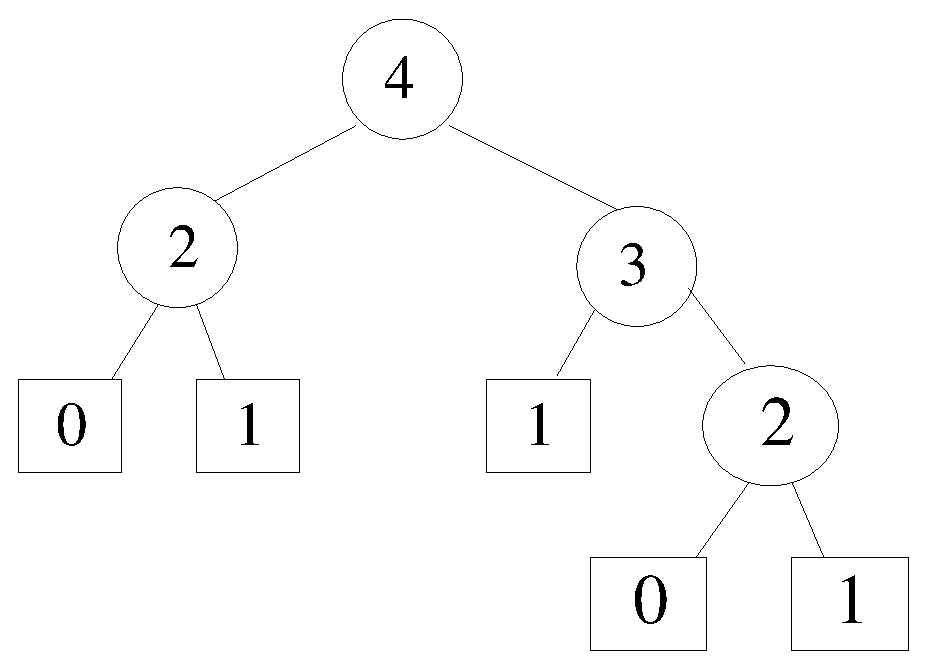
\includegraphics[width=0.35\linewidth]{arbreFibonacci.eps}
\end{center}

\Question{L'arbre de Fibonacci $T_4$ est dessin\'e ci-dessus. $T_0$ est une feuille portant l'\'etiquette 0,
$T_1$ est une feuille portant  l'\'etiquette 1; pour $n>1$, $T_n$ est un noeud binaire, dont le fils gauche est $T_{n-2}$ et dont le fils droit est $T_{n-1}$. Donnez une formule r\'ecursive pour 
le nombre total de noeuds (feuilles ou noeuds internes), not\'e $t_n$,  de $T_n$, pour $n>1$.}

\noindent{\bf Réponse}; $t_0=t_1=1$ et $t_n= t_{n-1} + t_{n-2}+1 $ pour $n>1$.

\Question{(suite) Donnez une formule récursive pour définir $u_n$ le nombre de feuilles \'etiquet\'ees 1 de $T_n$. Que constatez-vous?}

$u_n=u_{n-1} + u_{n-2}$ et $u_0=0, u_1=1$. La suite $u$ est donc la suite de Fibonacci.

\Question{(suite) Donnez une formule récursive pour définir  $z_n$ le nombre de feuilles \'etiquet\'ees 0 de $T_n$.}

$z_n= z_{n-1} + z_{n-2}$ et $z_0=1, z_1=0$. C'est la suite de Fibonacci à un décalage près. $z_n=u_{n-1}$.

\Question{(suite) Remplissez le tableau suivant, o\`u $u_n$ est le nombre de feuilles \'etiquet\'ees 1 de $T_n$,
$z_n$ le nombre de feuilles \'etiquet\'ees 0 de $T_n$, et $t_n$ le nombre de noeuds (feuilles ou non) de $T_n$.}

$$
\begin{array}{|c|c|c|c|c|c|c|c|c|c|c|}
\hline
n & 0 & 1 & 2 & 3 & 4 & 5 & 6 & 7 & 8 & 9 \\
\hline
t_n & 1 & 1 & 3 & 5 & 9 & 15 & 25 & 41 & 67 & 109  \\
\hline
u_n & 0 & 1 & 1 & 2 & 3 & 5 & 8 & 13 & 21 & 34  \\
\hline
z_n & 1 & 0 & 1 & 1 & 2 & 3 & 5 & 8 & 13 & 21   \\
\hline
\end{array}
$$
}

\Question{(suite) Donnez la formule matricielle pour calculer rapidement $t_n$.}

\noindent{\bf Réponse}.
$$(t_n, t_{n-1}, 1)=(t_{n-1},t_{n-2},1)\left( \begin{array}{ccc} 1 & 1 & 0 \\
1 & 0 & 0 \\
1 & 0 & 1 \end{array}\right)=(t_{1}, t_0, 1) \left( \begin{array}{ccc} 1 & 1 & 0 \\
1 & 0 & 0 \\
1 & 0 & 1 \end{array}\right)^{n-1}$$

Donc la méthode rapide pour la puissance de $G^{n-1}$, en $(\log n)$ multiplications, donne $t_n$.

Remarque. $t_n= 2u_{n+1}-1$, ce qu'on peut facilement prouver par récurrence.

\Question{Le temps d'ex\'ecution d'un algorithme  est
$T(n)$ pour une donn\'ee de taille $n$, o\`u $T(1)=1$ et $T(n)=3 T(n/2)+n$.
Prouvez en quelques lignes, par r\'ecurrence sur $k$, que $T(2^k) = 3^{k+1}-2^{k+1}$.
La formule est vraie pour $k=0$, ce qui permet d'amorcer la récurrence.}

\noindent{\bf Réponse}. Supposons la formule vraie jusqu'à $n=2^k$. 
Il faut la prouver pour $2n=2 ^ {k+1}$. Alors
$$T(2^{k+1})= 3 T(2^k)+2^{k+1}= 3 (3^{k+1}-2^{k+1}) + 2^{k+1}=3^{k+2} - 2^{k+2}$$ CQFD.

\Question{(suite) La complexité d'un algorithme est $T(2^k) = 3^{k}, n=2^k$. 
Déduisez-en la complexité de $T(n)$ en fonction de $n$~; vous la prouverez en une ligne~; les valeurs numériques de $\log_2 3$, ou autre, ne sont pas demandées. 
}

\noindent{\bf Réponse}. $k=\log_2 n$. La preuve suivante utilise~: $3=2 ^ {\log_2 3}$ et $ 2 ^ {\log_2 n}=n$.
$$T(n)=3^k = 3 ^{\log_2 n} = \left( 2 ^ {\log_2 3} \right) ^{\log_2 n} 
= 2^{(\log_2 3)\times (\log_2 n)} =  \left( 2 ^ {\log_2 n} \right) ^{\log_2 3}=n ^ {\log_2 3}= n^ {1.5849625007211563}$$

%%\end{multicols}
\end{document}
{
\Question{Un \'etudiant programme une m\'ethode de calcul de l'enveloppe convexe de $n$ points en 2D.
 Son programme met 1 seconde pour  $n=100$ mille points, et 8 secondes pour $n=200$ mille points. Son algorithme est en}
\begin{Reponse}
\Vrai $O(n^3)$; il s'agit vraisemblablement de la m\'ethode na\"ive qui teste toutes les paires de points pour d\'ecider si elle donne une ar\^ete de l'enveloppe convexe. 
\Faux $O(n^2)$
\Faux $O(n\log n)$
\Faux aucune des r\'eponses pr\'ec\'edentes n'est correcte.
\end{Reponse}
}

\Question{Prolongez de fa\c{c}on logique la suite de Fibonacci aux nombres n\'egatifs}
$$\begin{array}{|c|cccccccccccc|}
\hline
i & -6 & -5 & -4 & -3 & -2 & -1 & 0 & 1 & 2 & 3 & 4 & 5  \\
\hline
F_i & & & & & & & 0 & 1 & 1 & 2 & 3 & 5  \\
\hline
\end{array}
$$


\Question{Vous constatez que, pour $n\in \N$,  $F_{-2n}$ est \'egal \`a}

~\\

\Question{Vous constatez que, pour $n\in \N$,  $F_{-2n-1}$ est \'egal \`a}

~\\
 

\Question{Le temps d'ex\'ecution d'un algorithme  est
$T(n)$ pour une donn\'ee de taille $n$, o\`u $T(1)=1$ et $T(n)=3 T(n/2)+n$.
Prouver par r\'ecurrence que $T(2^k) = 3^{k+1}-2^{k+1}$}

~\\
~\\
~\\
~\\
~\\

\Question{Prouvez que $3^{\log_2 n}$ est en $O(n ^{log_3 2})$ (Remarque: $\log_3 2\approx 1.5849625$)}

~\\
~\\
~\\
~\\
~\\


\Question{Calculer le produit scalaire entre 2 vecteurs de $n$ nombres flottants $u=(u_i)$ et $v=(v_i)$ n\'ecessite}
\begin{Reponse}
\Faux $O(\log n)$ op\'erations flottantes
\Vrai $O( n)$ op\'erations flottantes
\Faux $O( n\log n)$ op\'erations flottantes
\Faux $O( n^2)$ op\'erations flottantes
\end{Reponse}

\Question{Calculer le produit entre une matrice carr\'ee quelconque de taille $n\times n$, contenant $n^2$  nombres flottants, et un vecteur colonne de $n$ \'el\'ements ($n$ nombres flottants)
n\'ecessite}
\begin{Reponse}
\Faux $O(n \log n)$ op\'erations flottantes
\Faux  $O(n )$ op\'erations flottantes
\Vrai  $O(n^2 )$ op\'erations flottantes
\Faux ce n'est pas toujours possible
\end{Reponse}

\Question{Calculer le produit entre deux matrices carr\'ees de taille  $n\times n$, en appliquant la formule~: $C_{lc}=\sum_{k=1}^n A_{lk}\times B_{kc}$, n\'ecessite}
\begin{Reponse}
\Faux $O(n \log n)$ op\'erations flottantes
\Faux  $O(n )$ op\'erations flottantes
\Vrai  $O(n^2 )$ op\'erations flottantes
\Vrai  $O(n^3 )$ op\'erations flottantes
\Faux ce n'est pas toujours possible (la matrice doit \^etre inversible, par exemple).
\end{Reponse}

\Question{La m\'ethode de puissance rapide pour calculer $M^k$ ($M$ est une matrice carr\'ee de taille $n\times n$, et $k$ est un entier naturel)  n\'ecessite}  
\begin{Reponse}
\Faux in\'evitablement $k-1$ (donc $O(k)$) multiplications de matrices carr\'ees de taille $n\times n$
\Vrai $O(\log k)$ multiplications de matrices carr\'ees de taille $n\times n$
\Vrai $O(k\log k)$ multiplications de matrices carr\'ees de taille $n\times n$
\Faux ce n'est pas toujours possible (la matrice doit \^etre inversible, par exemple).
\end{Reponse}


\Question{Trouver l'\'el\'ement le plus petit dans une liste non ordonn\'ee de taille $n>0$  n\'ecessite}
\begin{Reponse} 
\Faux $O(1)$ comparaisons
\Faux $O(n^2)$ comparaisons
\Vrai $O(n)$ comparaisons
\Faux $O(\log n)$ comparaisons
\end{Reponse} 

\Question{Trouver l'\'el\'ement le plus petit dans une liste tri\'ee par ordre croissant et de taille $n>0$  n\'ecessite}
\begin{Reponse} 
\Vrai $O(1)$ comparaisons
\Faux $O(n^2)$ comparaisons
\Vrai $O(n)$ comparaisons
\Faux $O(\log n)$ comparaisons
\end{Reponse}


\Question{
Un \'etudiant programme le tri rapide ("quicksort") d'une liste $L$ ainsi~: si $L$  contient moins de 2 \'el\'ements, alors elle est d\'ej\`a tri\'ee. Sinon, l'\'etudiant choisit un \'el\'ement $p$  dans $L$. Il partitionne $L$  
en 3 sous listes, la liste $L_1$ des \'el\'ements dans $L$ inf\'erieurs \`a $p$, la liste $L_2$ des \'el\'ements dans $L$
\'egaux \`a $p$,  
la liste $L_3$  des \'el\'ements dans $L$ sup\'erieurs \`a $p$. Il trie r\'ecursivement les 3 listes, puis concat\`ene les r\'esultats. 
Qu'en pensez-vous}
\begin{Reponse}
\Faux la m\'ethode est correcte mais la complexit\'e est modifi\'ee
\Faux la m\'ethode est correcte et la complexit\'e est inchang\'ee
\Vrai la m\'ethode est incorrecte ; elle boucle quand  $L$ contient deux (ou davantage) \'el\'ements \'egaux \`a $p$.
\Faux la m\'ethode est incorrecte car $L_2$ n'est jamais vide, puisqu'elle contient $p$.
\end{Reponse}


\Question{Pour le calcul de l'arbre couvrant minimum d'un graphe connexe, 
un \'etudiant propose l'algorithme suivant: si le graphe est un arbre, alors ins\'erer cet arbre dans l'arbre couvrant minimum;
sinon d\'ecomposer le graphe $G$ en 2 graphes de taille \`a peu pr\`es moiti\'e, $G_1$, et $G_2$, tous deux connexes; calculer
l'arbre couvrant minimum de $G_1$; calculer l'arbre couvrant minimum de $G_2$; joindre ces deux arbres par l'ar\^ete de co\^ut
 minimum entre $G_1$ et $G_2$ (cette ar\^ete a un sommet dans $G_1$ et un sommet dans $G_2$). 
Que pensez-vous de cet algorithme} 

\begin{Reponse}
\Faux il est correct
\Faux il est difficile de partitionner un graphe connexe en deux sous graphes connexes ayant (\`a peu pr\`es) deux fois moins de sommets; c'est pourquoi cet algorithme n'est pas utilis\'e
\Vrai il est incorrect, et voici un contre exemple simple (au plus 4 sommets!) :

~ \\
 ~ \\
~ \\
~ \\

\end{Reponse}


\Question{Une matrice de Vandermonde a la structure suivante~:
$$M= \left( \begin{array}{ccccc}
1 & 1 & 1 & \ldots & 1 \\
1 & w & w^2 & \ldots & w^{n-1} \\
1 & w^2 & w^4 & \ldots &  w^{2(n-1)} \\
\ldots & \ldots & \ldots & \ldots \\
1 & w^{n-1} &  w^{2n-2} &  \ldots & w^{(n-1)^2} \\
\end{array} \right)
$$ o\`u $n$ est une puissance de 2.
Si de plus $w$ est une racine $n$ i\`eme de l'unit\'e, alors le produit avec un vecteur colonne quelconque de taille $n$}
\begin{Reponse}
\Vrai peut se faire en $O(n \log n)$ (avec l'algorithme de la transform\'ee rapide de Fourier) 
\Vrai ne  peut pas se faire en moins que  $O(n)$
\Faux ne peut pas se faire en moins que $O(n^2)$
\end{Reponse}

\Question{Pour $n=8$ (donc $w^8=1$), \'ecrire la ligne de la matrice de Vandermonde commen\c{c}ant par $1$ puis  $w^3$, en simplifiant
(c'est \`a dire en \'eliminant les puissances plus grandes que 7)}

~\\
~\\
~\\
~\\

\Question{Idem, pour $n=8$, \'ecrire la ligne de la matrice de Vandermonde commen\c{c}ant par $1$ puis  $w^6$}

~\\
~\\
~\\
~\\

\Question{Dans le probl\`eme de la somme, un ensemble $E$ de $n$ entiers positifs $e_1 \ge e_2 \ge \ldots \ge e_n$ est donn\'e, ainsi
qu'un entier $0<S < \sum_1^n e_i$. Il faut trouver le sous ensemble $X$ de $E$ dont la somme des \'el\'ements
est maximum, mais inf\'erieure ou \'egale \`a $S$.  Pour tout ensemble $K$, on note $\sigma(K)$ la somme des \'el\'ements de $K$.
L'algorithme glouton calcule $X_0=\emptyset$ (donc $s(X_0)=0$);  puis, 
pour $i$ de 1 \`a $n$, il calcule $X_i= X_{i-1} \cup \{e_i\}$ si $e_i + \sigma(X_{i-1}) \le S$, et
$X_i= X_{i-1}$ sinon. Avec $E=100,25,20,10,1,1,1$ et $S=40$, donnez les valeurs de $X_0, X_1, \ldots X_7$, et les $\sigma(X_i)$ correspondants}

~\\
~\\
~\\
~\\
~\\
~\\
~\\

\Question{
Cet algorithme donne-t-il un sous ensemble $X_n$}
\begin{Reponse} 
\Vrai toujours correct ($s(X_n)\le S$), mais pas forc\'ement optimal : donnez un exemple simple ($n<5$) o\`u $X_n$ n'est pas optimal\\
~
\Faux toujours correct, et toujours optimal
\Faux pas toujours correct, mais optimal :  donnez un exemple simple ($n<5$) \\
~ 
\Faux souvent correct, et souvent optimal
\Faux ni correct ni optimal : donnez un exemple simple ($n<5$) \\
~
\Faux toutes les r\'eponses pr\'ec\'edentes sont fausses 
\end{Reponse}


\Question{Arthur conjecture que si, dans un graphe non orient\'e, tous les sommets distincts soit sont voisins, 
soit ont un voisin en commun, alors il existe au moins un sommet qui est voisin de tous les autres.  Que pensez vous de cette conjecture}
\begin{Reponse}
\Faux elle est vraie
\Vrai elle est fausse et vous en dessinez un contre exemple simple \\
~\\
\end{Reponse}


{

\Question{ Soient $\phi=\frac{1}{2}(1+\sqrt{5})\approx 1.618$ et $\phi'=\frac{1}{2}(1-\sqrt{5})\approx -0.618$~; ce sont les deux racines de $x^2-x-1=0$. 
D\'efinissons $f(n)=\frac{1}{\sqrt{5}}(\phi^n - \phi'^n)$.
Donnez la valeur de $f(0), f(1), f(2)$}\\
\noindent $f(0)=$\\
$f(1)=$\\
$f(2)=$\\

\Question{Par r\'ecurrence, prouvez que $F_n=f(n)$}

~\\
~\\
~\\
~\\
~\\
}
{
\Question{Quand un probl\`eme est dans NP, alors d\'ecider si une proposition de solution est vraiment solution est}
\begin{Reponse}
\Faux difficile  (d'o\`u la difficult\'e du probl\`eme)
\Vrai facile 
\end{Reponse}
}
{
\Question{Le tri bulle (bubble sort) \'echange deux \'el\'ements cons\'ecutifs qui ne sont pas dans le bon ordre, tant que c'est possible.
Donner l'ordre 
de grandeur du  nombre de permutations r\'ealis\'ees dans le  pire des cas.}
}
\end{multicols}
\end{document}
